\pagebreak
\section{Homography}

\subsection{Introduction}
In this assignment we were tasked to explore various applications of homographies. Like the first assignment, to obtain our goal we used Python and OpenCV as a toolkit. The purpose is to learn how to use homographies because it is related to both computer vision and computer graphics applications and is in general very useful for many applications. 

In this assignment we covered some uses of homographies like point transfers, texture mapping, camera calibration and some of the benefits of having a calibrated camera, however we cannot cover all of the homography uses because the time available for us is limited and there is extreme range of situations that homographies can be useful in.


\subsection{Person Map Location}

In this section, the task was to use linear algebra to map a person walk from video source taken at an angle to the overview map of the ITU. We have been given a video file where a person can be seen walking in the atrium of the IT University of Copenhagen, trace data that represents the person's position in each frame in the video, and an overview map of the ITU. We have also had a tool at our disposal that allowed us to obtain the homography matrix from the video to the map. 

We started by obtaining the homography matrix. We have specified four points in a frame of the provided video, and then we have tried to select the exact same points on the overview map. All of the four points had to lay on a plane, because a homography matrix describes the relation between two views of the same plane. We also need at least four points, because otherwise (e.g with three points) we would only be able to describe an affine transformation, not a projection. It is important to note, that since the entire video sequence of the walk is taken from a stationary camera (i.e the camera does not move during the exposition), and because the overview map of ITU is also not changing, it is sufficient to calculate the homography once for the entire sequence. Otherwise we would need to recalculate it for each frame when the relative position of the camera and the ground plane has changed.

\begin{figure}[h!]
	\centering
	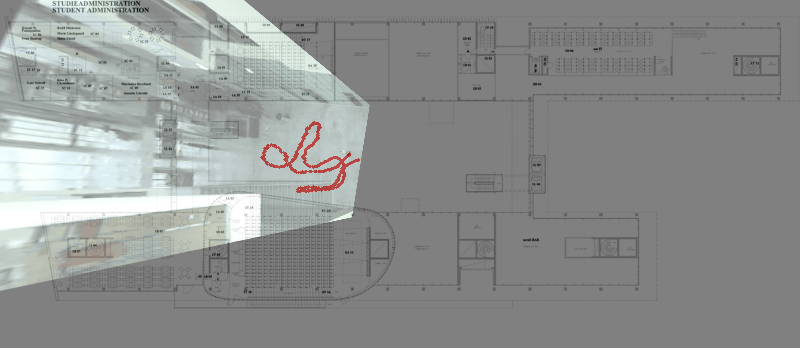
\includegraphics[width=\textwidth]{final/images/trace_map.png}
	\caption{Trace Map}
	\label{fig:trace}
\end{figure}

Using the obtained homography matrix we have been then able to project the video image onto the overview map of ITU which can be seen in the Figure \ref{fig:trace}. Using the provided trace data we have then been able to position the person in the overview map. We have taken the center point of the bottom edge of the rectangle describing the person's legs. This point should always be on the ground and therefore should guarantee the best approximation of the person's actual position (as opposed to the head for example, which would form a triangle between head, legs and a point defined by camera angle further away from the camera on the floor, yielding an inaccuracy of around the person's height at this camera angle).

\begin{equation}
	L = H \cdot P
	\label{form:homography}
\end{equation}

Figure \ref{fig:trace} has been produced by drawing a red point for each frame using the Formula \ref{form:homography} where L is the person's location in the overview map, H is the pre-calculated homography matrix, and P is a point corresponding to the middle of the bottom edge of the rectangle describing the person's legs.

\begin{figure}[h!]
	\centering
	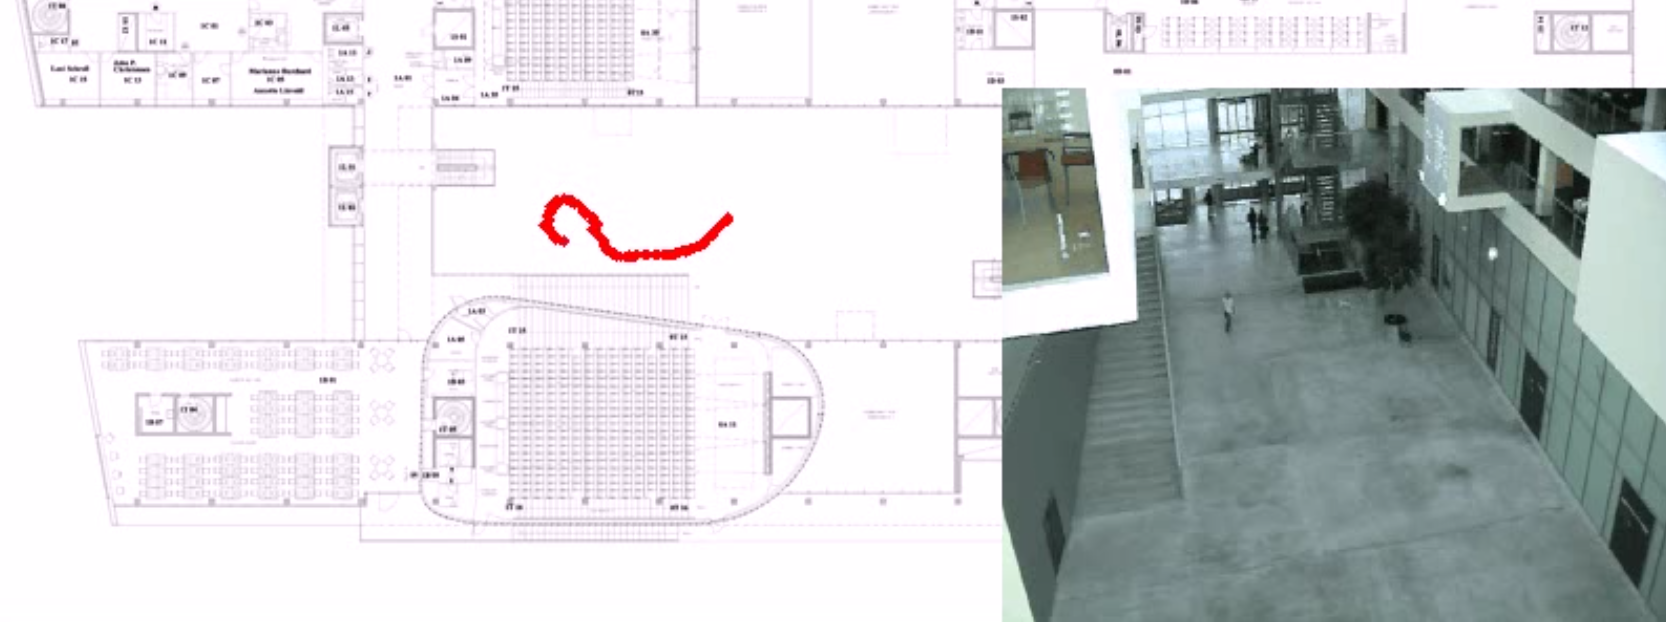
\includegraphics[width=\textwidth]{final/images/personlocationvideo.png}
	\caption{Video Trace}
	\label{fig:video_trace}
\end{figure}

The reason this mapping is useful, is that in the overview map it is easier to see the person's position on the ground plane. On the other hand, depending on the camera angle relative to the ground plane, the accuracy of the estimation can vary depending on the distance from the camera.

\subsection{Linear Texture Mapping}

This section is divided into three parts, first we will look at how to overview the ITU logo on the image sequence of universities ground floor. Then we look at how we can overview a texture on a moving object. In the third part we tried to be sure that the texture looks realistic compared to the geometry of the texture.

\subsubsection{Ground Floor}

In this part we tried to overview the ITU logo on the image sequence of ground floor. For this we used the same code from simpleTextureMap function and declare the texturemapGroundFloor method with the implementation for overviewing the logo on each frame of the sequence by using four mouse input points from the first frame.

\begin{figure}[h!]
	\centering
	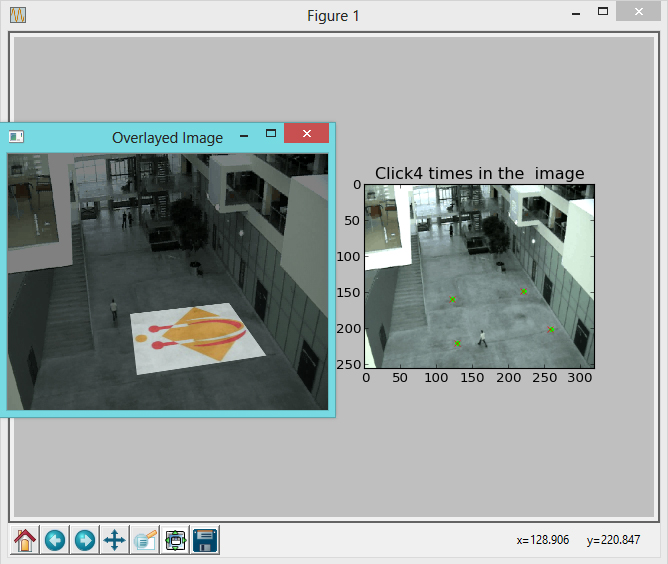
\includegraphics[width=\textwidth]{final/images/linearmapping.jpg}
	\caption{Linear Mapping}
	\label{fig:linearmapping}
\end{figure}

\subsubsection{Moving object}

In the second part of linear texture mapping we tried to experiment with texture mapping on image sequences where the objects move. We have been given some video files where a grid pattern moves in it. The aim is to mapping a texture on the pattern that will move with it. For the start we found the pattern corners with findChessboardCorners function and used it for calculating the homography matrix and overview the logo on the pattern. So for each frame we get a new homography matrix and new texture mapping. Our implementation weakness is that in some frames that it cannot detect corners of the pattern it will fail because we used corners location to mapping the logo.

\begin{figure}[h!]
	\centering
	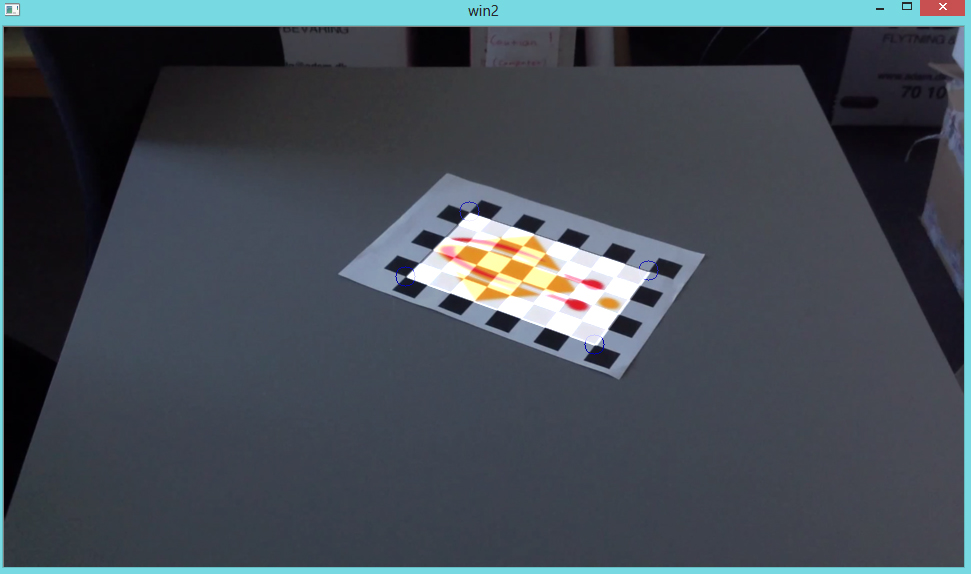
\includegraphics[width=\textwidth]{final/images/linearmapping2.jpg}
	\caption{Moving Pattern}
	\label{fig:movingpattern}
\end{figure}

\subsubsection{Ensuring a correctly placed texturemap}

The last part, depicted in Figure \ref{fig:realistictexturing}, is realistic texture placement on the ground floor. We start by selecting a point in the overview map. Next, we calculate placement of corner points in the overview map. We regard the selected point as a center, and then we calculate the corners from provided scale factor and texture dimensions.

We are then able to obtain the positions of the corners in the video image by calculating the dot product of the inverse of the homography $H_{G}^{M}$ and the positions of the points in the overview map. We can then calculate the homography between the texture T and ground plane in the video image G $H_{T}^{G}$. This allows us to position the texture consistently with the ground plane just by selecting a single point.

\begin{figure}[h!]
	\centering
	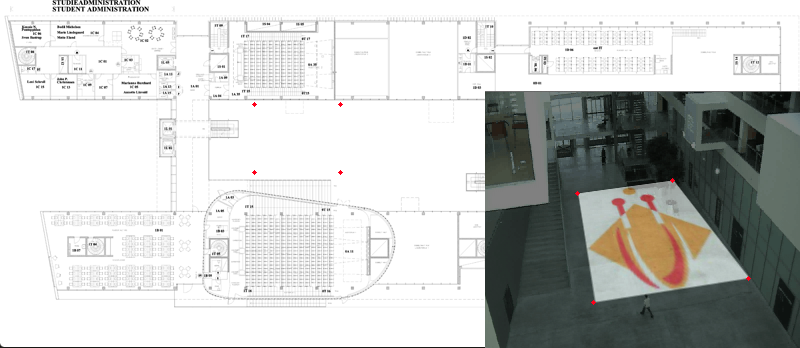
\includegraphics[width=\textwidth]{final/images/realistictexturing.png}
	\caption{Realistic Texturing}
	\label{fig:realistictexturing}
\end{figure}

\subsection{Camera Calibration and Augmentation}

This section is divided into two parts, first we will look at how we obtained proper camera calibration and distortion coefficients. Then we look at how we used this information to augment the image obtained from the camera with a projected cube.

\subsubsection{Camera Calibration}

During the camera calibration phase we aim to obtain intrinsic camera parameters. This is divided into two parts, first there is a camera matrix K (see Equation \ref{eq:cameramatrix}) which describes the intrinsic properties of the camera, and then there are distortion coefficients which we do not represent in the linear camera model, but they affect the image nonetheless. 

The R|t part is the rotation/translation matrix. These are the extrinsic properties of the camera like its rotation and translation in the world.

P is a point in the 3D space that we want to project onto the 2D image obtained by the camera. 

C represents the 2D coordinates in the image produced by the camera when P is projected.

\begin{equation}
	\underbrace{
		\begin{bmatrix}
			u \\
			v \\
			1
		\end{bmatrix}
	}_\text{C}
	=
	\underbrace{
		\begin{bmatrix}
			f_{x} & 0 & t_{x} \\
			0 & f_{y} & t_{y} \\
			0 & 0 & 1
		\end{bmatrix}
	}_\text{K}
	\cdot
	\underbrace{
		\begin{bmatrix}
			R_{1,1} & R_{1,2} & R_{1,3} & t_{x} \\
			R_{2,1} & R_{2,2} & R_{2,3} & t_{y} \\
			R_{2,1} & R_{2,2} & R_{3,3} & t_{z}
		\end{bmatrix}
	}_\text{R|t}
	\cdot
	\underbrace{
		\begin{bmatrix}
			X \\
			Y \\
			Z \\
			1
		\end{bmatrix}
	}_\text{P}
	\label{eq:cameramatrix}
\end{equation}

The calibration is obtained in OpenCV by repeated exposures containing the calibration pattern. Based on this, OpenCV calculates the intrinsic camera properties and returns them as K and distortion coefficients. It should be noted that unless the camera allows for focal length manipulation, the intrinsics will not change. So it makes sense to just calibrate once and save the calibration into a file which then can be reused.

\subsubsection{Augmentation}

In the next part we have used the calibration obtained in the previous section to augment the image with a 3D object (cube) Figure \ref{fig:augment}. The basis for this was to obtain a homography from one virtual camera to another. 

\begin{figure}[h!]
	\centering
	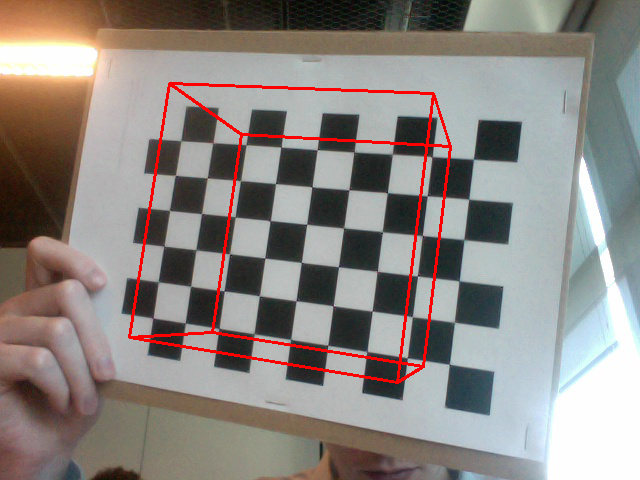
\includegraphics[width=\textwidth]{final/images/augmentation1.png}
	\caption{Augmented image}
	\label{fig:augment}
\end{figure}

First we have constructed a camera that would look at just the chessboard pattern. Then we have calculated the positions of some select corners in that pattern, and using the same corners in the same pattern in the image obtained from the video, we have been able to estimate a homography that would describe the relationship between the two.

From that we have been able to re-construct the camera that was essentially used to take the video image. we have had the calibration from before, and now using the homography we have been able to calculate the rotation and translation matrices from the Equation \ref{eq:solvingforrotation} where we obtain $r_{1}$, $r_{2}$ and t as dot product of the inverse of K, the calibration matrix, and H, the homography between the two planes. $r_{3}$ can be calculated as a cross product of $r_{1}$ and $r_{2}$.

\begin{equation}
	K^{-1}H = [r_{1}, r_{2}, t]
	\label{eq:solvingforrotation}
\end{equation}

Now using the projection matrix of the second camera, we can project points in the 3D space onto the final image, so that they appear as if they were in the scene. And since the homography is calculated from one chessboard to another, the points are anchored the position of the chessboard.

\subsection{Conclusion}
In the beginning we started with the point transfers and texture mapping, by detecting a person movement and overviewing an image in a video with using homography. The challenges we faced in this part were to working with matrixes and points in images and sequences. We tried to implement fast and optimized codes to get the best result and reduce the wrong results and code failure in video frames.

Next, we worked on camera calibration and some of the benefits of having a calibrated camera like augmented reality. The biggest challenge was to understand in what order should we apply the homographies to the points to draw them on the screen.

We had a successful achievement on working with homographies and its usage. Texture mapping and augmentation were really excitement and useful and surely in the future more developers are going to use these technics in their applications.

